\documentclass[border=10pt]{standalone}
\usepackage[T1]{fontenc}
\usepackage{lmodern}
\usepackage{tikz}
\usetikzlibrary{shapes.geometric, arrows.meta, positioning}

\begin{document}
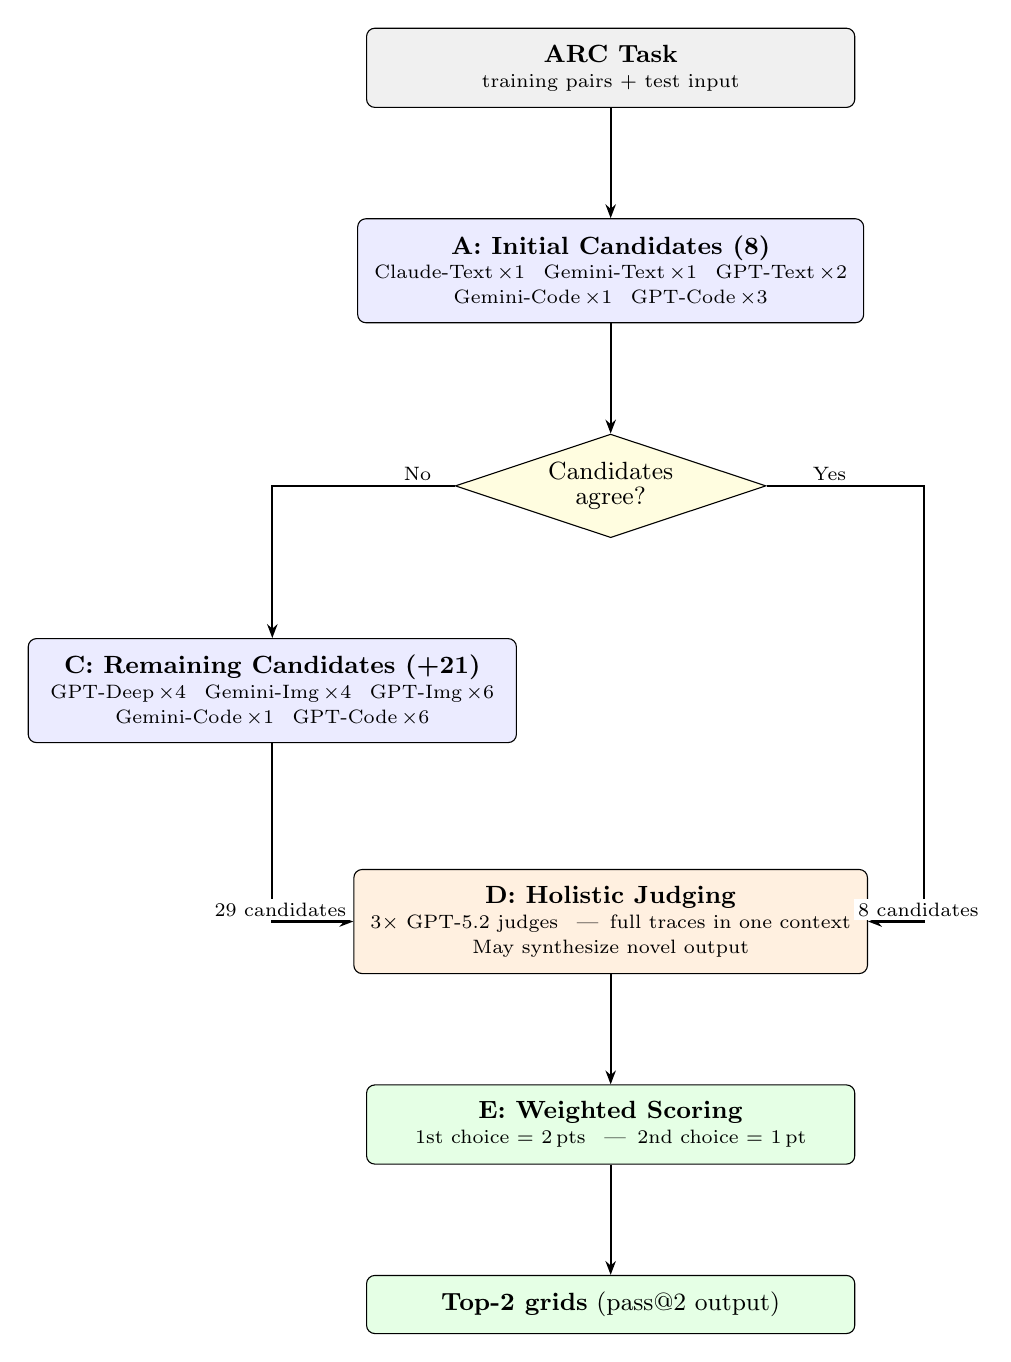
\begin{tikzpicture}[
    node distance=1.4cm,
    box/.style={rectangle, draw, rounded corners=3pt, minimum width=6.2cm, align=center, font=\small, inner sep=6pt},
    inputbox/.style={box, fill=gray!12},
    stepbox/.style={box, fill=blue!8},
    judgebox/.style={box, fill=orange!12},
    outputbox/.style={box, fill=green!10},
    diam/.style={diamond, draw, aspect=3.0, fill=yellow!12, align=center, font=\small, inner sep=2pt},
    arr/.style={-{Stealth[length=5pt]}, thick},
    lbl/.style={font=\scriptsize, fill=white, inner sep=1.5pt},
]

% Nodes
\node[inputbox] (task) {\textbf{ARC Task}\\[-2pt]{\scriptsize training pairs + test input}};

\node[stepbox, below=of task] (stepA) {\textbf{A: Initial Candidates (8)}\\[-2pt]
{\scriptsize Claude-Text\,$\times$1 \enspace Gemini-Text\,$\times$1 \enspace GPT-Text\,$\times$2}\\[-2pt]
{\scriptsize Gemini-Code\,$\times$1 \enspace GPT-Code\,$\times$3}};

\node[diam, below=of stepA] (stepB) {Candidates\\[-2pt]agree?};

\node[stepbox, below left=1.6cm and 0.2cm of stepB] (stepC) {\textbf{C: Remaining Candidates (+21)}\\[-2pt]
{\scriptsize GPT-Deep\,$\times$4 \enspace Gemini-Img\,$\times$4 \enspace GPT-Img\,$\times$6}\\[-2pt]
{\scriptsize Gemini-Code\,$\times$1 \enspace GPT-Code\,$\times$6}};

\node[judgebox, below=4.2cm of stepB] (stepD) {\textbf{D: Holistic Judging}\\[-2pt]
{\scriptsize 3$\times$ GPT-5.2 judges \enspace|\enspace full traces in one context}\\[-2pt]
{\scriptsize May synthesize novel output}};

\node[outputbox, below=of stepD] (stepE) {\textbf{E: Weighted Scoring}\\[-2pt]
{\scriptsize 1st choice = 2\,pts \enspace|\enspace 2nd choice = 1\,pt}};

\node[outputbox, below=of stepE] (output) {\textbf{Top-2 grids} {\small (pass@2 output)}};

% Arrows
\draw[arr] (task) -- (stepA);
\draw[arr] (stepA) -- (stepB);

% No branch
\draw[arr] (stepB.west) -| node[lbl, pos=0.05, above left] {No} (stepC.north);
\draw[arr] (stepC.south) |- node[lbl, pos=0.55, above] {\scriptsize 29 candidates} (stepD.west);

% Yes branch
\draw[arr] (stepB.east) -- ++(2.0,0) node[lbl, pos=0.4, above] {Yes} |- node[lbl, pos=0.55, above] {\scriptsize 8 candidates} (stepD.east);

\draw[arr] (stepD) -- (stepE);
\draw[arr] (stepE) -- (output);

\end{tikzpicture}
\end{document}
